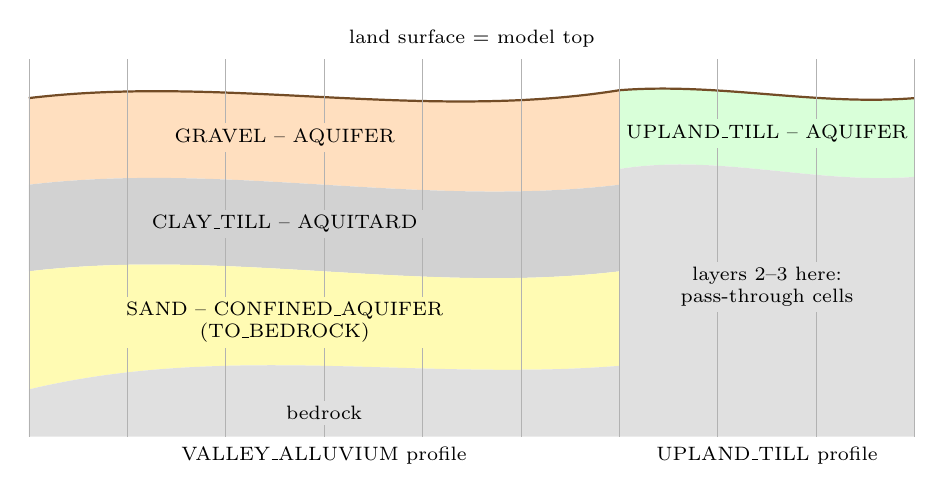
\begin{tikzpicture}[x=1.25cm,y=1.0cm,lab/.style={font=\scriptsize,align=center,inner sep=2pt}]
\fill[orange!25] (0,4.3) .. controls (2,4.6) and (4,4.0) .. (6,4.4) -- (6,3.2) .. controls (4,2.9) and (2,3.5) .. (0,3.2) -- cycle;
\fill[gray!35] (0,3.2) .. controls (2,3.5) and (4,2.9) .. (6,3.2) -- (6,2.1) .. controls (4,1.8) and (2,2.4) .. (0,2.1) -- cycle;
\fill[yellow!30] (0,2.1) .. controls (2,2.4) and (4,1.8) .. (6,2.1) -- (6,0.9) .. controls (4,0.7) and (2,1.2) .. (0,0.6) -- cycle;
\fill[black!12] (0,0.6) .. controls (2,1.2) and (4,0.7) .. (6,0.9) -- (6,0) -- (0,0) -- cycle;
\fill[green!15] (6,4.4) .. controls (7,4.5) and (8,4.2) .. (9,4.3) -- (9,3.3) .. controls (8,3.2) and (7,3.6) .. (6,3.4) -- cycle;
\fill[black!12] (6,0) -- (6,3.4) .. controls (7,3.6) and (8,3.2) .. (9,3.3) -- (9,0) -- cycle;
\draw[thick,brown!60!black] (0,4.3) .. controls (2,4.6) and (4,4.0) .. (6,4.4) .. controls (7,4.5) and (8,4.2) .. (9,4.3);
\foreach \x in {0,1,...,9} \draw[gray!60,very thin] (\x,0) -- (\x,4.8);
\node[lab,fill=white,inner sep=1pt] at (4.5,5.05) {land surface = model top};
\node[lab,fill=orange!25] at (2.6,3.8) {GRAVEL -- \cmd{AQUIFER}};
\node[lab,fill=gray!35] at (2.6,2.7) {CLAY\_TILL -- \cmd{AQUITARD}};
\node[lab,fill=yellow!30] at (2.6,1.45) {SAND -- \cmd{CONFINED\_AQUIFER}\\ (\cmd{TO\_BEDROCK})};
\node[lab,fill=black!12] at (3.0,0.3) {bedrock};
\node[lab,fill=green!15] at (7.5,3.85) {UPLAND\_TILL -- \cmd{AQUIFER}};
\node[lab,fill=black!12] at (7.5,1.9) {layers 2--3 here:\\ pass-through cells};
\node[lab,anchor=north] at (3,-0.05) {\cmd{VALLEY\_ALLUVIUM} profile};
\node[lab,anchor=north] at (7.5,-0.05) {\cmd{UPLAND\_TILL} profile};
\end{tikzpicture}
